% !TeX spellcheck = en_US
\addscenariosection{1}{Clash Scenario}{King of the Hill}{\images/kingofthehill.png}

\begin{multicols*}{2}

\textbf{Author:} LAAMAKALA

\textit{In the battle for the Hill, there is no honor — only victory or death. The weak will fall, the strong will fight, and only one will rule.}

\subsection*{\MakeUppercase{Scenario Length}}
This Scenario plays out over 8 Rounds.

\subsection*{\MakeUppercase{Player Setup}}
\textbf{Player Count:} 2 -- 4

\textbf{Starting Resources:} 15 \svg{gold}, 2 \svg{building_materials}, 1 \svg{valuables}

\textbf{Starting Income:} 10 \svg{gold}, 2 \svg{building_materials}, 1 \svg{valuables}

\textbf{Starting Units:}
\begin{itemize}
  \item Few of \silver\ with the lowest Recruitment cost.
  \item 1 random Neutral \bronze\ Unit.
\end{itemize}

\textbf{Town Buildings:}
\begin{itemize}
  \item \bronze\ Dwelling
  \item City Hall
  \item \svg{building_special_tent} Building
\end{itemize}

\subsection*{\MakeUppercase{Map Setup}}
Take the following Map Tiles and arrange them as shown in the Scenario map layout ($P$ stands for the number of players):

\begin{itemize}
  \item P × Starting (I) Map Tile
  \item 2P × Far (II-III) Map Tiles
  \item 2P × Near (IV-V) Map Tiles
  \item 1 × Center Map Tile. The center Field is ``The Hill''
\end{itemize}

\subsection*{\MakeUppercase{Victory Conditions}}
The game ends at the end of Round 8.

\subsection*{\MakeUppercase{Victory Points}}
The player with the most Victory Points (VP) wins (see Tournament Book). players also gain:
\begin{itemize}
  \item 5VP for the first player flagging ''The Hill''
  \item 2VP at the end of every Round for the player who controls ''The Hill''
  \item 1VP for losing a Combat against another player
\end{itemize}

\subsection*{\MakeUppercase{Timed Events}}

\begin{itemize}
  \item \textbf{\nth{1} Round:} all Heroes gain +1 \svgeven{movement}.
  \item \textbf{\nth{2} Round:} Players may gain either 10 \svg{gold}, 4 \svg{building_materials} or 2 \svg{valuables}.
  \item \textbf{\nth{5} Round:} Remove all black Cubes.
  \item \textbf{\nth{7} Round:} all Heroes gain +1 \svgeven{movement}.
\end{itemize}

\subsection*{\MakeUppercase{Additional Rules}}
\begin{itemize}
  \item Remove ``Unexpected Reinforcements'' from the Astrologers Proclaim Deck.
  \item \azure\ Units cannot be recruited at any point of the game.
  \item Citadel cannot be built on Round 1.
  \item The blocked Field on the Center Map Tile is a Magic Spring and does not count as blocked.
  \item All Fields on Center Map Tile are visitable once per Faction.
  \item Players do not lose gold for losing or retreating from any Combat.
  \item \textbf{Sanctuary:} Empower a Knowledge Statistic Card \textit{OR} gain +1 \svg{morale_positive}. \textit{Visitable once per Faction.}
  \item \textbf{Obelisk:} Draw 1 Card. \textit{Visitable once per Faction.}
  \item \textit{Optional:} At the beginning of each Round, roll two Attack Dice separately and apply the effect from the table below.
\end{itemize}

\hommtablemulticol[]{33}{
  \centering
  \medskip
  \textbf{Battlefield Conditions}\\ 
  \medskip

  \begin{tabularx}{0.95\linewidth}{p{0.15\linewidth}XXXX}\\
  \darkcell[1.4]{-1/-1}
    & \lightcell[1.4]{Dense Fog – All Ranged Units gain disadvantage.}\\
  \darkcell[1.4]{-1/0}
    & \lightcell[1.4]{Raining Ash – All \svg{unit_flying-table} Units gain -2 \svg{initiative-table}.}\\
  \darkcell[1.4]{0/-1}
    & \lightcell[1.4]{Sinking Mud – All \svg{unit_ground-table} Units move one space less.}\\
  \darkcell[1.4]{-1/+1}
    & \lightcell[1.4]{Scorching Earth – All \silver\ and \golden Units start Combat with 1 \svg{damage-table}.}\\
  \darkcell[1.4]{0/0}
    & \lightcell[1.4]{Clear Skies – No effect.}\\
  \darkcell[1.8]{+1/-1}
    & \lightcell[1.8]{Fey Trickery – Players Activate their Units in ascending order of Unit Initiative.}\\
  \darkcell[1.4]{0/+1}
    & \lightcell[1.4]{Rocky Terrain – All Ground Units gain \svg{defense_yellow} Token.}\\
  \darkcell[1.4]{+1/0}
    & \lightcell[1.4]{Tail Wind – \svg{unit_flying-table} Units gain +1 Movement.}\\
  \darkcell[1.4]{-1/-1}
    & \lightcell[1.4]{Perfect Conditions – All \svg{unit_ranged-table} Units gain advantage.}\\
  \end{tabularx}
}
\begin{itemize}
  \item After winning a Neutral Combat, you may sacrifice 3 \bronze\ Units to gain 1 \silver\ Unit you defeated.
  \item At the start of next turn, a defeated main Hero may gain +2 \svg{movement}, Empower any Statistic Card from their M\&M Deck AND Search (2) the \silver\ Neutral Deck.
\end{itemize}

\begin{center}
  \vfill
  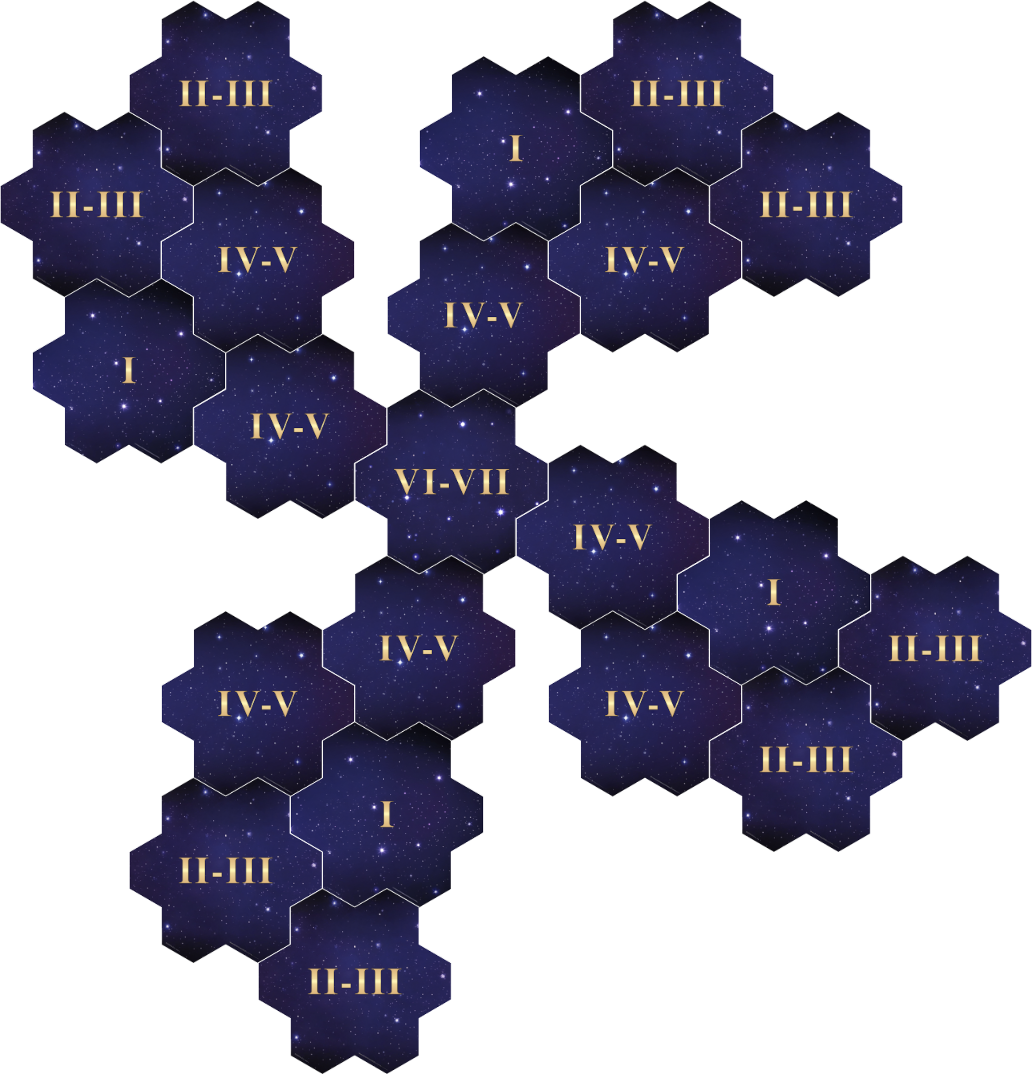
\includegraphics[width=1.0\linewidth]{\maps/king_of_the_hill-2.4p.png}
  \captionof{figure}{\textbf{2/4-PLAYER SCENARIO}}
  \vfill
  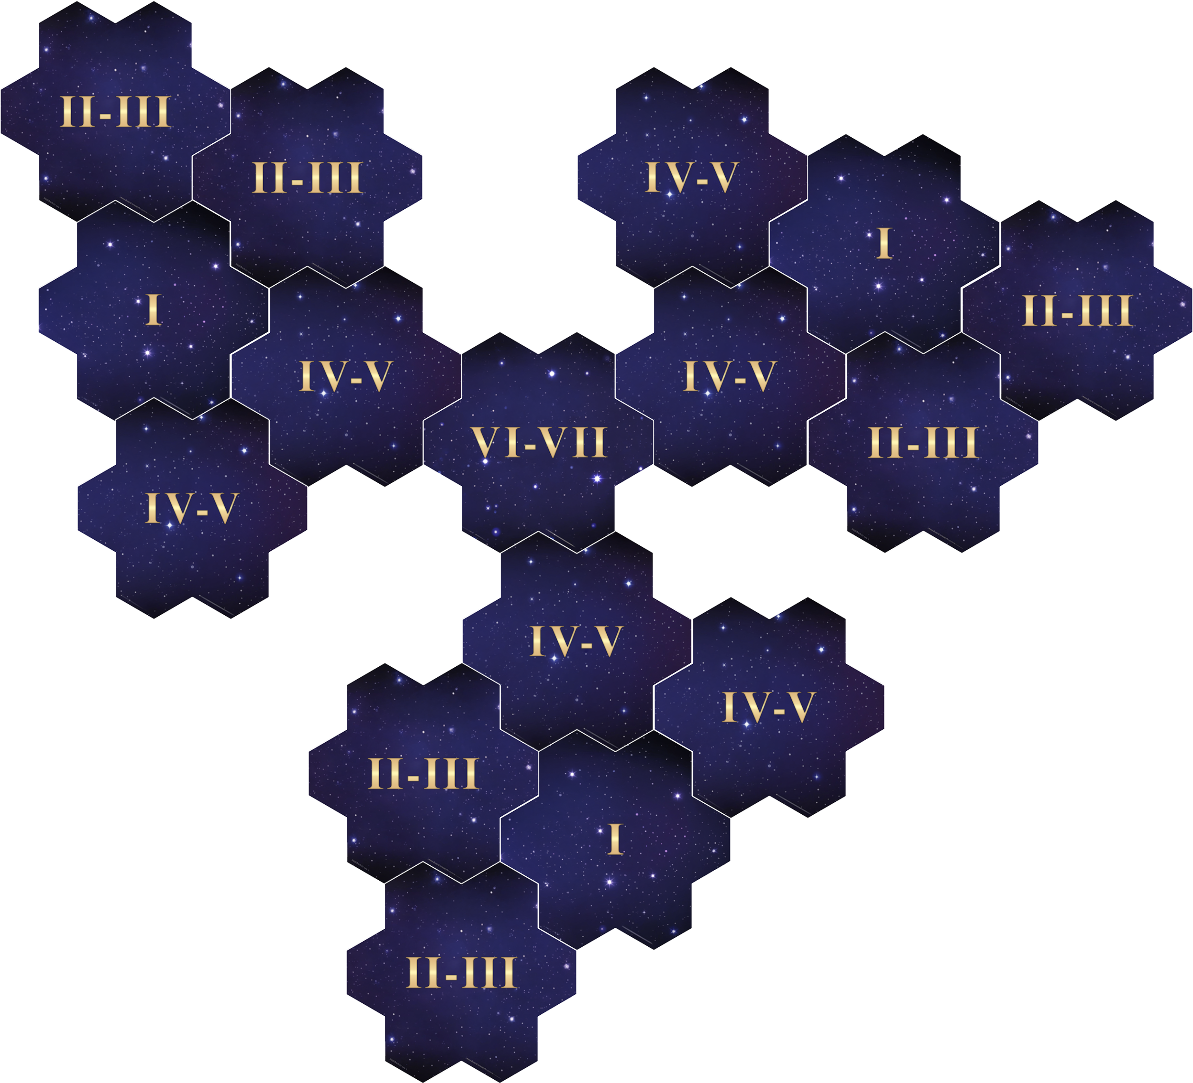
\includegraphics[width=1.0\linewidth]{\maps/king_of_the_hill-3p.png}
  \captionof{figure}{\textbf{3-PLAYER SCENARIO}}
\end{center}

\end{multicols*}